\chapter{Technical and Legal Background}

This chapter presents the technical foundations of browser extension development and the relevant European Union laws for compliance auditing. We provide a general overview here, while the detailed technical implementation of CookieAudit is discussed in \cref{ch:implementation}.

\section{Browser Extensions}
%We implemented CookieAudit as a browser extension.
%To understand the implementation details in \cref{ch:implementation}, we will give an overview of the architecture and implementation of browser extensions.

Browser extensions are programs that can extend or change the functionality of browsers.
They are built using web technologies (JavaScript, HTML, CSS) and can use the APIs provided by the browser.
The APIs of Chromium-based browsers (e.g., Chrome and Edge) overlap in large parts with the APIs of Mozilla's Firefox, while Apple's Safari sometimes differs significantly.
As a result, many extensions can run in several browser environments.

When building browser extensions for Chromium-based browsers, developers have to split up their code according to the specification by Manifest Version 3~\cite{manifestv3}.
In this section, we first explain the different parts of a general browser extension architecture and then detail the challenges posed by Manifest V3.
\cref{fig:extension-architecture} shows a visualization of the building blocks and their interactions.

\begin{figure}
	\centering
	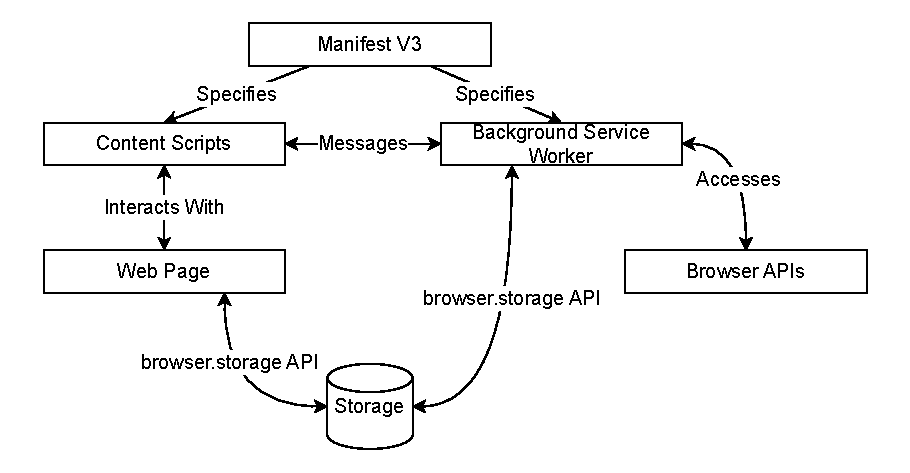
\includegraphics[width=\textwidth]{media/browser-extension-architecture.drawio.pdf}
    \caption{The general architecture of a manifest version 3 browser extension.}
    \label{fig:extension-architecture}
\end{figure}

\subsection{Extension Service Workers} \label{subsec:service-workers}
The Extension Service Worker is the central location for business logic.
By having access to the full WebExtensions API, it is the place to define event listeners,\footnote{
By registering event listeners at the beginning of the service worker, developers can define code that should handle events.
The most relevant events are browser events (e.g., first installation of an extension), tab events (e.g., user navigating to a different URL), and extension events (e.g., messaging between extension components).}
send and receive messages to and from the content scripts and popup
or run time intensive computations~\cite[Ch. 4]{frisbie2023browser}.
Service workers operate asynchronously on a separate thread, preventing interference with website execution. 
They are ephemeral, started by event handlers and terminated when idle.
Therefore, developers must persist important application state to storage (see \cref{subsec:storage}) rather than relying on in-memory variables, as these are reset upon termination.

\subsection{Content Scripts} \label{subsec:content-scripts}
Content scripts are JavaScript programs injected into web pages. 
They can access and modify the page's HTML structure and CSS styles.
By default, content scripts run in an isolated environment, separate from the page's own JavaScript.\footnote{
Developers can deactivate this isolation by setting the execution world to \texttt{MAIN}. Then, the content script will be able to, e.g., read variables of the web page JavaScript.
}
This isolation prevents direct access between the content script and page script.
Variables are not shared, and functions from one context cannot be called by the other.
Content scripts have limited access to the WebExtensions API, for example, they cannot change the current tab's URL.
To interact with the rest of the extension, content scripts use messaging and a shared key-value store.

\subsection{Communication}
Since the extension service worker and the different content scripts run in separate JavaScript environments, variables and functions cannot be accessed across those boundaries.
Instead, browsers provide the messaging API to send and listen for messages.
For example, in the context of cookie notice detection, if a content script has detected a cookie notice and needs to inform the extension service worker about it, one could send a corresponding message as in \cref{fig:message-passing}.

\begin{figure}
	\centering
	\definecolor{backcolour}{rgb}{0.95,0.95,0.92}
	\lstset{backgroundcolor=\color{backcolour}}
	    
	\begin{subfigure}{\textwidth}
		\centering
		\begin{lstlisting}
let response = await chrome.runtime.sendMessage({
  cookieNoticeDetected: true
});
		\end{lstlisting}
		\caption{Sending a message from the content script}
	\end{subfigure}
	    
	\begin{subfigure}{\textwidth}
		\centering
		\begin{lstlisting}
function handleMsg(request,sender,sendResponse) {
  // ... handle message inside request object ...
  // send response to content script:
  sendResponse({ storedData: true });
}
chrome.runtime.onMessage.addListener(handleMsg);
		\end{lstlisting}
		\caption{Handling a message in the background script}
	\end{subfigure}
	    
	\caption{Message passing in Chrome extension}
	\label{fig:message-passing}
\end{figure}

\subsection{Storage} \label{subsec:storage}
Browser extensions often need to be able to store data across browser restarts.
Developers can therefore use the asynchronous\footnote{Even though JavaScript is single-threaded, its asynchronous mechanisms allow non-blocking execution, handling tasks like I/O operations without halting the main thread.} storage API to store key-value pairs serialized as JSON objects. Serializable types include primitives, arrays, and objects\footnote{
Associative arrays, also known as maps or dictionaries, are called objects in JavaScript.
}, but not functions or DOM elements (\texttt{HTMLElement}).

\subsection{Popup}
The primary way for users to interact with a browser extension is through a small dialog called \emph{popup}.
It can only be opened by the user, that is, by clicking the extension’s action icon in the browser toolbar.
Popups are programmed using the same web technologies as websites: HTML, CSS, and JavaScript. 
They have access to all WebExtensions APIs provided by the browser, e.g., storage and messaging. 
\cref{fig:screenshot-popup} shows the popup of CookieAudit.

\begin{figure}
	\centering
	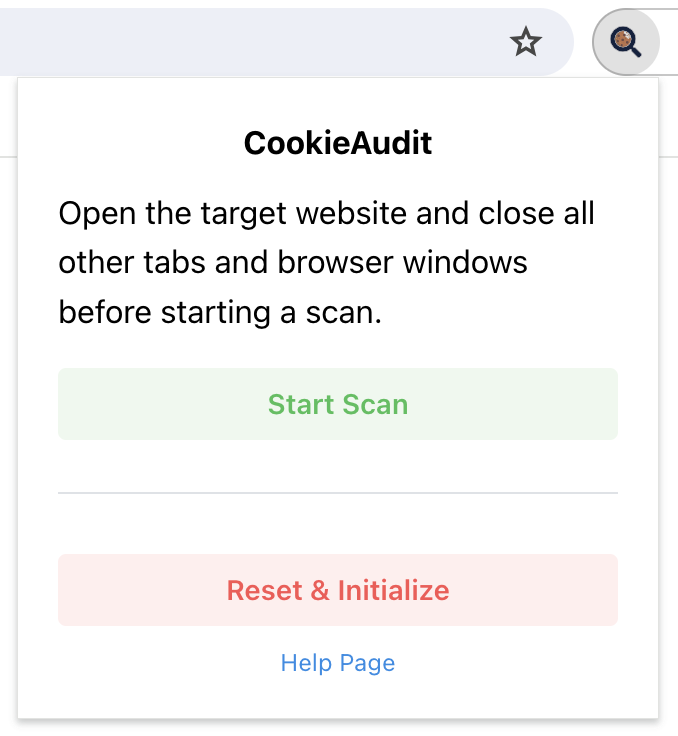
\includegraphics[width=0.5\linewidth]{screenshot_popup.png}
	\caption{Popup dialog of CookieAudit}
	\label{fig:screenshot-popup}
\end{figure}

\subsection{Manifest Version 3} \label{subsec:manifest-v3}
We developed CookieAudit according to Manifest version 3~\cite{manifestv3}.
It is the newest specification of the extensions API for Chromium-based browsers.
Compared to Manifest version 2, it includes API changes and restrictions aimed to increase the security and performance of extensions.
Version 3 has forced some developers to make considerable changes to their extensions~\cite{purdy2024chrome, huczynski2018ublock}, sometimes even reducing the functionality~\cite{hill2024google}.
We present some notable changes between Manifest versions 2 and 3.

\subsubsection{From background scripts to service workers}
In Manifest version 2, developers could use \texttt{background scripts} which effectively were non-visible, persistent web pages.
Many extensions developed for manifest version 2 used the fact that background scripts are never terminated and that their global variables are accessible from the extension popup.
As explained in \cref{subsec:service-workers}, developers cannot rely on those characteristics anymore.
The migration to manifest version 3 sometimes required considerable changes in the architecture of extensions.\footnote{
For example, Gonzalez reported increased complexity following the move of the Bitwarden password manager to Manifest V3~\cite{gonzalez2024bitwarden}.
The switch to service workers made changes in the extension architecture necessary.}
Furthermore, the mechanism requiring idle service workers to restart after being shut down can lead to delays in event handling.
This time to revival can be problematic for time sensitive extensions.

\subsubsection{Execution of arbitrary Strings}
The execution of arbitrary strings with the \texttt{eval()} function could be used for security exploits, as shown by Carlini et al.~\cite{carlini2012evaluation}.
To solve this issue, it is no longer possible to evaluate and execute strings using methods such as \texttt{eval()}, or \texttt{new Function()}.
It is still possible to evaluate and execute WebAssembly,\footnote{WebAssembly is a binary instruction format designed as a fast, safe compilation target for languages like C/C++. It provides JavaScript interoperability and runs in web browsers~\cite{haas2017wasm}.} by specifying \texttt{wasm-unsafe-eval} in the extension manifest.
The ability to run WebAssembly is necessary for many performance critical applications, such as the client-side inference of AI models.

\subsubsection{Other}
Manifest version 3 introduces several other significant changes to browser extension development.
It limits the inspection and modification of live network requests and prohibits the execution of remotely hosted code.\footnote{
All code must be included within the extension package which is published in the extension stores.
}
Furthermore, the new version renames and restructures some WebExtensions API functions.

%\color{orange}
\section{Cookies}
HTTP Cookies are small pieces of text data stored in a user's browser when visiting websites. 
They are initially created by web servers, sent to clients, and stored by browsers. 
Each cookie is associated with a specific domain.
\emph{First-party} cookies are associated with the domain of the website being visited.
For example, when visiting \texttt{news.example}, a cookie may be set with that same domain.
\emph{Third-party} cookies are associated with domains different from the website being visited. 
For instance, if \texttt{news.example} displays an advertisement served from \texttt{ads.example}, the ad server can set cookies with the \texttt{ads.example} domain.
Cookies are automatically sent back to their originating servers with every HTTP request to that domain. 
This adds state to the otherwise stateless nature of HTTP.

Cookies serve various purposes. 
They can provide essential functionality, such as storing user authentication data. 
However, they can also be used to track users across different websites for analytics or advertising purposes.
This is done by creating a unique, identifying key for each user and storing it as a cookie.

\section{General Data Protection Regulation and ePrivacy Directive} \label{sec:legal}
The General Data Protection Regulation (GDPR) and the ePrivacy Directive (ePD) govern data collection and processing in the European Union (EU).
The GDPR defines the data subject (user), controller (typically a website operator), processor (e.g., a cloud provider), and third parties as key entities involved in data collection and processing.
It regulates controllers within the EU as well as those who handle the personal data of EU residents.
Both laws only regulate personal data, which is specifically defined in Article 4 of the GDPR as any information related to an \enquote{identified or identifiable natural person}.
Browser cookies that are not strictly necessary to provide the service, on the other hand, are covered by Article 5(3) of the ePD.
The article requires user consent for storing and accessing data on the users' device, unless strictly necessary for providing a service~\cite{kubicek2024phd}.

For a controller to lawfully process personal data, at least one of the six possible legal bases defined in Article 6 of the GDPR must be satisfied.
These legal bases include consent, contractual necessity, legal obligation, vital interests, public interest, and legitimate interests.
However, in the particular context of websites using personal data and cookies for monetization, only the basis of user consent can be used~\cite{kubicek2024phd}.
Consent must be a \enquote{freely given, specific, informed, and unambiguous indication of the data subject's agreement to the processing of personal data relating to him or her} (Recital 32 of the GDPR).
This implies that consent on websites has to be a voluntary choice by the subject, with equal ease for acceptance and rejection (\emph{freely given}), should always be tailored to a single collection and processing purpose (\emph{specific}), based on clearly communicated practices of data collection and processing (\emph{informed}), and explicitly provided by the user, such as by clicking on a checkbox or signing up for a newsletter (\emph{unambiguous})~\cite{kubicek2024phd}.

Non-compliance with the GDPR can result in severe penalties. 
Supervisory authorities can impose fines of up to €20 million or 4\% of the organization's global annual turnover, whichever is higher~\cite{sanchez_rola2019can}. 
